\chapter{Motivation}

In 2001 Alexei Yu. Kitaev presented a model for implementing qubits
that could face the problem of high decoherency in quantum computation \citep{kitaev_unpaired_2001}. Kitaev's idea was centered in using the properties of an exotic quasi-particle that appears at the edges of a quantum superconducting chain. This quasi-particle receives the name of Majorana Fermion, is characterized for being its own anti-particle, thus it has no charge or spin. It also presents non-Abelian statistics, a desired property to implement fault-tolerant quantum computers\citep{kitaev_fault-tolerant_2003}. These majorana fermions where theoretically predicted since the 1930's by one of the genius of the era, Ettore Majorana \citep{wilczek_majorana_2009}.
Although no fundamental Majorana-particle has been discovered to the
date, Kitaev's model inspired the pursue of majorana fermions as
quasi-particles in a novel exotic class of materials known as topological
superconductors (TS)\citep{fu_superconducting_2008,sato_non-abelian_2009,alicea_new_2012}.
\\

The last five years have been full of excitement, as new experiments
have turned some of the theoretical predictions of the 1990s and 2000s
into a reality. Very recently the first evidence of Majorana end states
in TS has been found in multiple experiments \citep{mourik_signatures_2012,das_zero-bias_2012,deng_anomalous_2012}
following the prescription by \citet{oreg_helical_2010} and \citet{lutchyn_majorana_2010}.
These experiments have been based on tunneling spectroscopy in junctions
between TS and non metallic (NM) leads, where resonances have been
observed at zero energy, consistent with the presence of Majorana
zero\textendash energy modes.\\

A downside of the tunneling spectroscopy technique in this case, is
that it probes not only the end of the Topological Superconductor(TS), but its bulk as well ,
which completely destroys the qubit information. A less destroying
model presented by \citet{liu_detecting_2011} consists in coupling
a quantum dot (QD) to the end of a TS, and carrying out transport
measurements on the QD itself. The analysis performed by Liu of this
model revealed a drop in the conductance peak of $\frac{e^{2}}{2h}$
when the TS is in the topological phase, making this a signature of
Majorana physics. Later, \citet{vernek_subtle_2014} showed that this
phenomena was the consequence of leaking of the Majorana Bound State
(MBS) at the edge of the TS into the QD. \\

Inspired by these results, in a paper published by my former advisor
and coauthors \citep{ruiz-tijerina_interaction_2015}, \citeauthor{ruiz-tijerina_interaction_2015}
studies a more general QD model that includes the spin degree of freedom
and local Coulomb interactions. At low temperatures these interactions produce strong correlations
between the NM electrons through the QD state, producing a phenomenon
known as the Kondo effect \citep{hewson_kondo_1997}. This effect
is characterized by the formation of a very particular many-body ground state given by
a singlet entangling the QD spin and the NM band. This results in the emergence of a zero-mode with high density of states which enhances the QD conductance at zero-bias.


The results of this paper finally show that transport measurements
through the quantum dot will show contributions to the enhanced conductance
coming from the Kondo effect and the Majorana mode: The Majorana mode
at the end of the wire will migrate into one of the QD spin channels,
giving rise to a zero\textendash energy peak in the density of states
(\ref{Fig-Kondo-Majorana conductance}a)) contributing a conductance
of $\frac{e^{2}}{2h}$(\ref{Fig-Kondo-Majorana conductance}c)). The
zero\textendash bias peak from the Kondo effect appears in the other
spin channel (\ref{Fig-Kondo-Majorana conductance}b)), contributing
a conductance of $\frac{e^{2}}{h}$. Then, the Kondo effect can be
\textquotedblleft turned off\textquotedblright{} through gate voltages
and magnetic fields, leaving only the Majorana contribution. Clear
evidence of the destruction of the Kondo peak will appear in the conductance,
allowing for a distinction between Majorana and Kondo signatures.\\



 Apart from not destroying the entire qubit-information the QD-method has another insight.  This is the possibility of "moving" around Majoranas  in multidot systems by shifting the QD gate voltages and tunnel couplings. Hence the approach is suitable for the implementation of braiding procedures. The simplest system where Majorana manipulation is possible is  a  Double Quantum Dot (DQD) coupled to a majorana chain. By tuning the QD gate voltages and the majorana coupling we will be able to probe the mobility of the majorana modes through the dots. 
 
 When both dots are coupled to the leads the Double Quantum Dot exhibits an antiferromagnetic interaction known as  Ruderman-Kittel-Kasuya-Yosida (RKKY) interaction\cite{ruderman_indirect_1954,kasuya_theory_1956,yosida_magnetic_1957}. On the other hand, when only one QD is coupled to the leads and the other Dot is attached to the QD,  the Kondo effect is annihilated due to the destructive interference  generated by extra dot \cite{dias_da_silva_transmission_2008}. Our study includes how the Majorana mode interacts with these two effects.  
The final aim of this project is to generalize this model to executing
transport measurements through $2$-QDs coupled to a TS. This study
will be performed using numerical calculations of the many-body spectrum
of the system with with Wilson\textquoteright s Numerical Renormalization
Group (NRG) technique \citep{wilson_renormalization_1975}. The increasing
number of arrangements of the new model will worth for the study of
new physics such as the possible braiding\citep{kitaev_fault-tolerant_2003}
of both majoranas in the TS. 


\begin{figure}[ht]
\centering
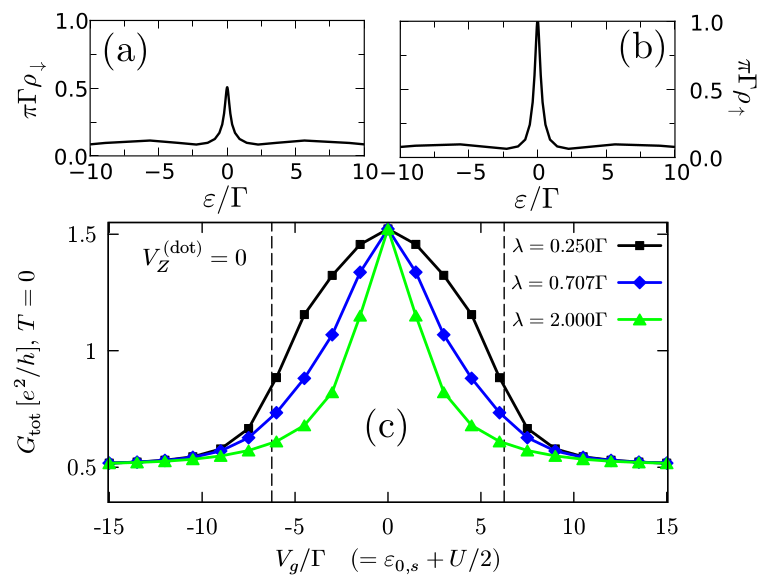
\includegraphics[scale=0.4]{IMAGES/Kondo-Majorana Conductivity.png}
\caption{\label{Fig-Kondo-Majorana conductance}(a) QD spin-down
density of states. Because this channel couples to the Majorana mode,
it displays the characteristic zero-bias signature of amplitude
$\frac{e^{2}}{2h}$. (b) QD spin-up density of states,
displaying the zero-bias peak of the Kondo effect, with
unit amplitude. (c) Zero-bias conductance of the QD coupled
to the Majorana mode, as a function of the QD energy level ($\lambda$
parameterizes the strength of the Majorana-QD tunnel coupling).
The presence of the spin-up Kondo resonance enhances the
QD conductance in particle-hole symmetry ($V_{g}=0$),
but quickly disappears as the QD level is detuned from this point.
The spin-down Majorana signature, on the other hand, is
robust {[}7{]}, leaving a residual conductance of $\frac{e^{2}}{2h}$.
Extracted from \citep{ruiz-tijerina_interaction_2015}.}
\end{figure}



